
\documentclass{beamer}

\usepackage[utf8]{inputenc}
\usepackage[english]{babel}
\usepackage{amsmath}
\usepackage{graphicx}
\usepackage{placeins}
\usepackage{pgffor}
\usepackage{hyperref}
\usepackage{subcaption}
\usepackage[T1]{fontenc}
\usepackage{algpseudocode}
\usepackage{pythontex}
\usepackage{xcolor}

\definecolor{velvet}{rgb}{0.67058824, 0.08235294, 0.16862745}
\definecolor{offwhite}{rgb}{0.90, 0.90, 0.90}
\usetheme{Montpellier}
\setbeamercolor{palette primary}{bg=offwhite,fg=white}
\setbeamercolor{frametitle}{fg=black}


%%%% headline %%%%
\setbeamercolor{section in head/foot}{bg=velvet}
\setbeamercolor{separation line}{bg=offwhite}

\useoutertheme[subsection=false]{miniframes}

\title{\color{velvet}
	Particle swarm optimisation\\with the use of chaos maps
	}
\author{
Piedebout Laurent,
Habbal Younes,
Demangeon Antoine,
Choiset Flore
}
\date{03 juin 2022}



\begin{document}

	%page de présentation
	\begin{frame}
	\titlepage
	\end{frame}


	\begin{frame}
	\frametitle{\color{velvet} Introduction and motivations}
	\framesubtitle{What is optimisation?}
		\begin{center}
		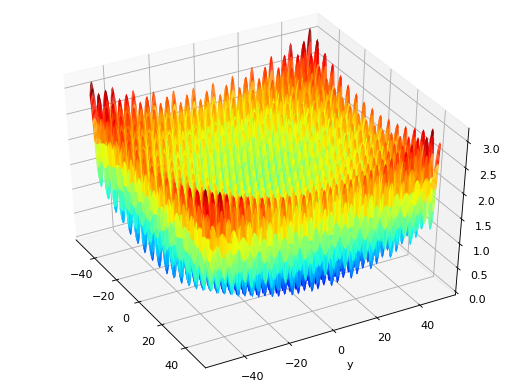
\includegraphics[scale=0.45]{optimisation.png}
		\end{center}
	\end{frame}
%L'optimisation est un enjeu essentiel dans de nombreux secteurs tels que l'informatique, les mathématiques, l'ingénieurie mais aussi l'économie et la physique. 
%On cherche à apporter à chaque problème la meilleure approximation possible de la solution. Pour décrire ce problème, on définit une fonction cherche à minimiser ou à maximiser par rapport à tous les paramètres concernés. 
%Optimiser une situation revient donc à rechercher le minimum ou le maximum de la fonction qui la décrit. 
%Cependant, dans certaines situations on peut trouver une grande quantité d'extremums locaux. Ces derniers ne nous interessent pas et peuvent même poser problème, la solution recherchée correspondant à un extremum global. 
%La définition d’un problème d’optimisation est souvent complétée par des contraintes : tous les paramètres des solutions retenues doivent respecter ces contraintes, faute de quoi ces solutions ne sont pas réalisables.

	\begin{frame}
	\frametitle{\color{velvet} Introduction and motivations}
	\framesubtitle{PSO algorithm}
	
		\begin{center}
		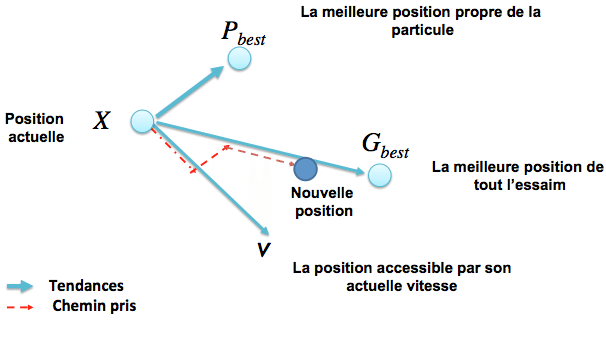
\includegraphics[scale=0.45]{graphPSO.png}
		\\James Kennedy and Russel Eberhart, 1995
		\end{center}
	\end{frame}

%La méthode PSO fait partie de la famille algorithmique des métaheuristiques. 
%Les métaheuristiques sont généralement des algorithmes stochastiques itératifs, qui progressent vers un extremum global visant ainsi à résoudre des problème d'optimisation. 
%Les premières recherches sur cet algo datent de 1995 et ont été réalisée par James Kennedy et Russel Eberhart. 
%Elles sont inspirées d'observation faites sur des vols d'oiseaux et des bancs de poissons. 
%Ces observations ont révélées la capacité des individus d’un groupe en mouvement à conserver une distance optimale entre eux et à suivre un mouvement global par rapport aux mouvements locaux de leur voisinage. 
%D’autre part, ces observations ont également révélé des phénomènes de mimétisme entre les individus d'un groupe. 
%Chaque individu cherche à optimiser ses chances en suivant une tendance qu’il modère par ses propres vécus. 
%L’optimisation par essaim de particules repose donc sur un ensemble d’individus appelés particules qui se déplacent dans l'espace de recherche et construisent une solution au problème posé en s'appuyant sur leur inertie, leur expérience personnelle et leur expérience collective.

\begin{frame}
	\frametitle{\color{velvet} Algorithm}
	\framesubtitle{Computation method}
	
		\begin{center}


			$V_{k+1} = \omega_v V_k + r_1 \omega_l (P_{local best} - P_{k}) + r_2 \omega 
			_g (P_{global best} - P_{k})$
			\\[0.2cm]

			$X_{k+1} = X_k + V_{K+1}$
			\\[0.2cm]

			%with omegav in [0,1]
			%and r1 in [0,1] , computed thanks to the chaos function

			$\omega_v \in [0,1]$,
			$r_1 \in [0,1]$,
			$r_2 \in [0,1]$\\
			$r_1$ and $ r_2 $ are computed using the chaos map
			
			\vspace*{0.5cm}

			%add a matrix of the position of 10 particles in n dimensions
			%add a matrix of the velocity of 10 particles in n dimensions

			\scalebox{0.75}{
			\begin{math}
				P_k =
				\begin{bmatrix}
					x_{1,1} & x_{2,1} & x_{3,1} & x_{4,1} & \dotsm  & x_{q,1} \\
					x_{1,2} & x_{2,2} & x_{3,2} & x_{4,2} & \dotsm & x_{q,2} \\
					x_{1,3} & x_{2,3} & x_{3,3} & x_{4,3} & \dotsm & x_{q,3} \\
					\multicolumn{6}{c}{$\vdots$}     				\\
					x_{1,n} & x_{2,n} & x_{3,n} & x_{4,n} & \dotsm & x_{q,n}
				\end{bmatrix}
			\end{math}
				;
			\begin{math}
				V_k =
				\begin{bmatrix}
					x_{1,1} & x_{2,1} & x_{3,1} & x_{4,1} & \dotsm  & x_{q,1} \\
					x_{1,2} & x_{2,2} & x_{3,2} & x_{4,2} & \dotsm & x_{q,2} \\
					x_{1,3} & x_{2,3} & x_{3,3} & x_{4,3} & \dotsm & x_{q,3} \\
					\multicolumn{6}{c}{$\vdots$}     				\\
					x_{1,n} & x_{2,n} & x_{3,n} & x_{4,n} & \dotsm & x_{q,n}
				\end{bmatrix}
			\end{math}
			}



		\end{center}
\end{frame}

\begin{frame}
	\frametitle{\color{velvet} Algorithm}
	\framesubtitle{Computation method}
	
				\begin{algorithmic}
					\State $k_{max} \gets n$
					\State $i \gets 0$
					\State $X_{k} \gets X_0$
					\State $X_{kminlocal} \gets X_k$
					\State $X_{kminglobal} \gets min(X_{kminlocal})$
					\While{$ ERX(X_k) \geq \epsilon \, and \, i \leq k_{max}$} 
						\State $V_{k} \gets \omega_v V_{k-1} + r_1(i) \omega_l (P_{local best} - P_{k})$
						\State $V_{k} \gets V_{k} + r_2(i) \omega_g (P_{global best} - P_{k})$
						\State $X_{k} \gets X_{k-1} + V_{k}$
						\State $X_{kminlocal} \gets min(X_{k})$
						\State $X_{kminglobal} \gets min(X_{kminlocal})$
						\State $i \gets i + 1$
					\EndWhile
				\end{algorithmic}

\end{frame}
		
\foreach \i in {0,1,2,3,4,5,6,7,8,9,10,11,12,13,14,15,16,17,18,19,20}{
	\begin{frame}
		\begin{center}
			\frametitle{\color{velvet}Rastrigin function}
			\includegraphics[scale=0.5]{rastigin/\i.png}	
		\end{center}
	\end{frame}
}
	
\foreach \i in {0,1,2,3,4,5,6,7,8,9,10}{
	\begin{frame}
		\begin{center}
			\frametitle{\color{velvet}Booth function}
			\includegraphics[scale=0.5]{booth/\i.png}	
		\end{center}
	\end{frame}
}


	

%Younes work / Part 3

\begin{frame}
	%Comparaison entre les ERJ obtenues avec une chaos map et une loi uniforme}
	\frametitle{\color{velvet}Comparison between the ERJ obtained with a chaos map and a uniform distribution}
	%Evolution d'ERJ en fonction de D
	\framesubtitle{Evolution of ERJ in regard of the dimension}
	Evolution of ERJ in regard of the dimension
	\includegraphics[scale=0.7]{uniforme/erreur_en_fct_de_D.png}
\end{frame}
	
\begin{frame}
	\frametitle{\color{velvet}Comparison between the ERJ obtained with a chaos map and a uniform distribution}
	\framesubtitle{Evolution of ERJ in regard of the log(K)}
	Evolution of ERJ in regard of the $log(K)$
	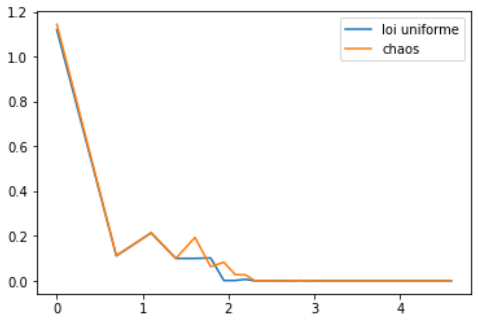
\includegraphics[scale=0.7]{uniforme/erreur_en_fct_de_logK.png}
\end{frame}
	
\begin{frame}
	\frametitle{\color{velvet}Comparison between the ERJ obtained with a chaos map and a uniform distribution}
	\framesubtitle{Evolution of ERJ in regard of the log(P)}
	Evolution of ERJ in regard of the $log(P)$
	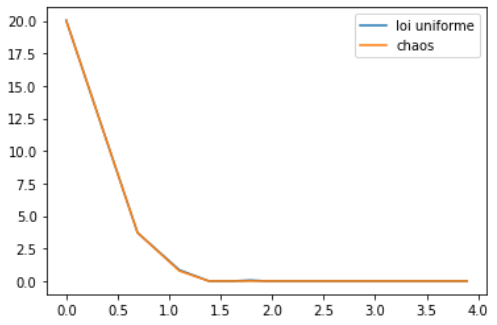
\includegraphics[scale=0.7]{uniforme/erreur_en_fct_de_logP.png}
\end{frame}

\begin{frame}
	\frametitle{Algorithm}
	\framesubtitle{Generating rk using the standard normal distribution}
	rk is a n-sized vector containing random values generated with a standard normal distribution,
	\begin{algorithmic}
					\State $X_{min} \gets min(rk)$
					\State $X_{max} \gets max(rk)$
					\State $i \gets 0$
					\While{$ i < n $}
						\State $rk[i] \gets (rk[i]-X_{min})/(X_{max}-X_{min})$
						\State $i \gets i + 1$
					\EndWhile
				\end{algorithmic}
	
	\end{frame}
	
\begin{frame}
	\frametitle{\color{velvet}Comparison between the ERJ obtained with a chaos map and a normal distribution}
	\framesubtitle{Evolution of ERJ in regard of the value of D}
	Evolution of ERJ in regard of the value of D
	\includegraphics[scale=0.7]{normale/erreur_en_fct_de_D.png}
\end{frame}
	
\begin{frame}
	\frametitle{\color{velvet}Comparison between the ERJ obtained with a chaos map and a normal distribution}
	\framesubtitle{Evolution of ERJ in regard of the log(K)}
	Evolution of ERJ in regard of the $log(K)$
	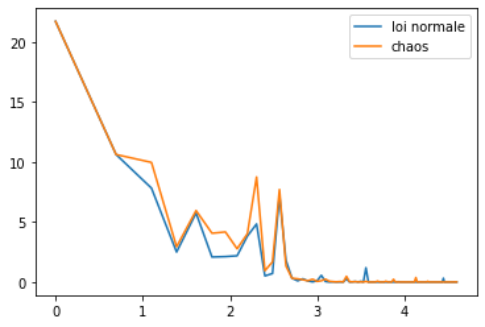
\includegraphics[scale=0.7]{normale/erreur_en_fct_de_logK_3.png}
\end{frame}
	
\begin{frame}
	\frametitle{\color{velvet}Comparison between the ERJ obtained with a chaos map and a normal distribution}
	\framesubtitle{Evolution of ERJ in regard of the log(P)}
	Evolution of ERJ in regard of the $log(P)$
	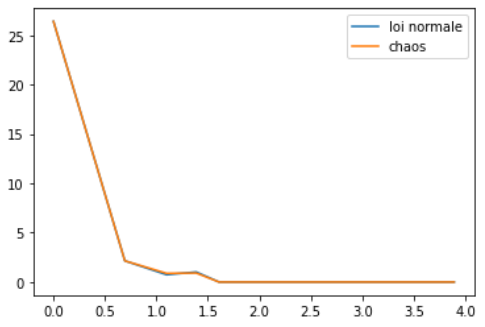
\includegraphics[scale=0.7]{normale/erreur_en_fct_de_logP_2.png}
\end{frame}

%Python generated, see the python script displaygraph / Part 4
\begin{frame}
	\frametitle{\color{velvet} Study of the impact of the parameters on the convergence}
	\framesubtitle{Evolution of ERJ in regard of the number of dimensions | Dimension 2}
	The value of the final ERJ is: 0.017894385917374578
	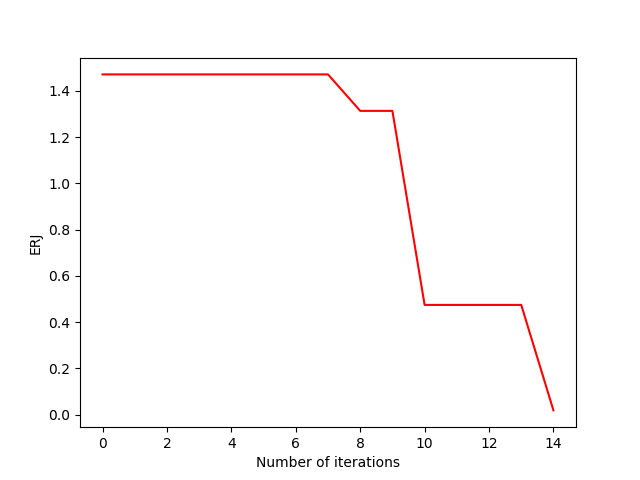
\includegraphics[scale=0.5]{Graphs/1.png}
	\end{frame}
	\begin{frame}
	\frametitle{\color{velvet} Study of the impact of the parameters on the convergence}
	\framesubtitle{Evolution of ERJ in regard of the number of dimensions | Dimension 5}
	The value of the final ERJ is: 2.9848775024190743
	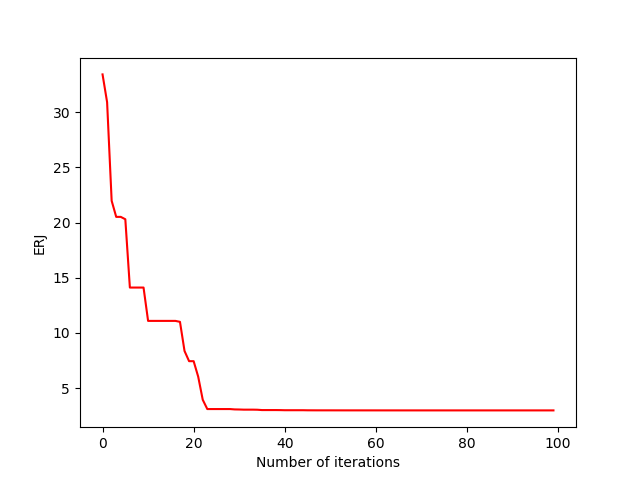
\includegraphics[scale=0.5]{Graphs/2.png}
	\end{frame}
	\begin{frame}
	\frametitle{\color{velvet} Study of the impact of the parameters on the convergence}
	\framesubtitle{Evolution of ERJ in regard of the number of dimensions | Dimension 10}
	The value of the final ERJ is: 4.014968644746489
	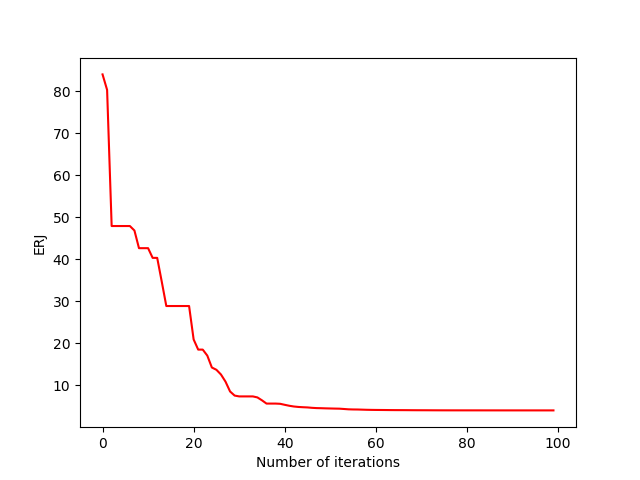
\includegraphics[scale=0.5]{Graphs/3.png}
	\end{frame}
	\begin{frame}
	\frametitle{\color{velvet} Study of the impact of the parameters on the convergence}
	\framesubtitle{Evolution of ERJ in regards of the number of dimensions | Dimension 50}
	The value of the ERJ is: 205.75578243398908
	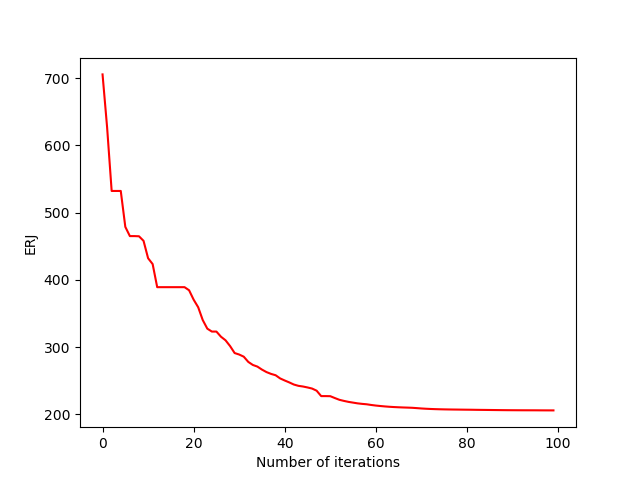
\includegraphics[scale=0.5]{Graphs/4.png}
	\end{frame}
	\begin{frame}
	\frametitle{\color{velvet} Study of the impact of the parameters on the convergence}
	\framesubtitle{Evolution of ERJ in regards of the number of dimensions | Dimension 100}
	The value of the ERJ is: 562.2491221239749
	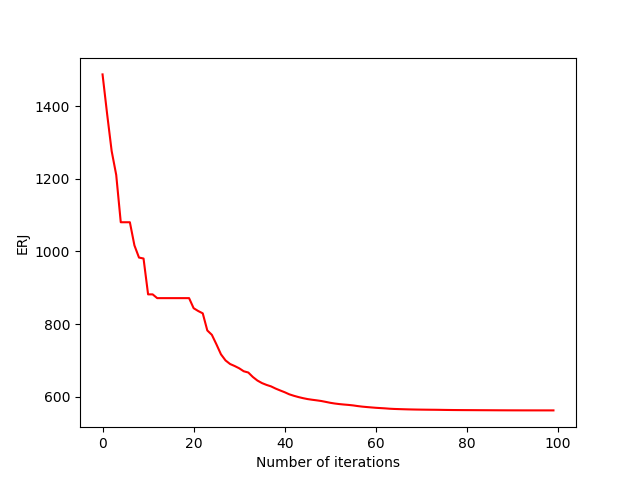
\includegraphics[scale=0.5]{Graphs/5.png}
	\end{frame}
	\begin{frame}
	\frametitle{\color{velvet} Study of the impact of the parameters on the convergence}
	\framesubtitle{Evolution of ERJ in regard of the dimension}
	The higher the dimension, the higher the ERJ is
	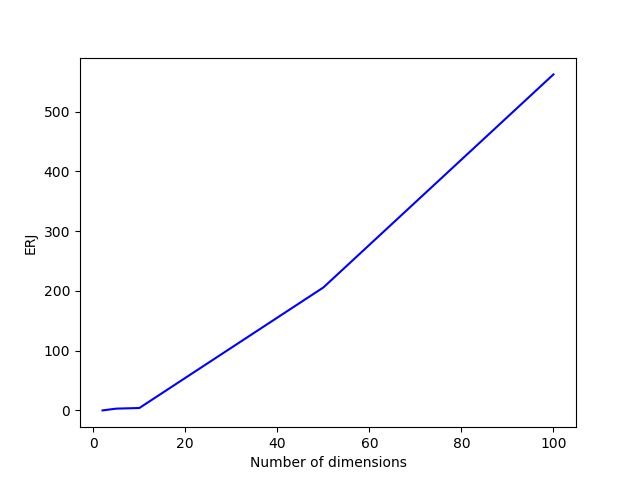
\includegraphics[scale=0.5]{Graphs/6.png}
	\end{frame}

	%partie laurent
\begin{frame}
	\frametitle{Study of the impact of the parameters on the convergence}
	\framesubtitle{Optimisation in higher dimensions (above five)}
		\begin{columns}
    		\column{7cm}
    			\begin{figure}
      				\centering
       				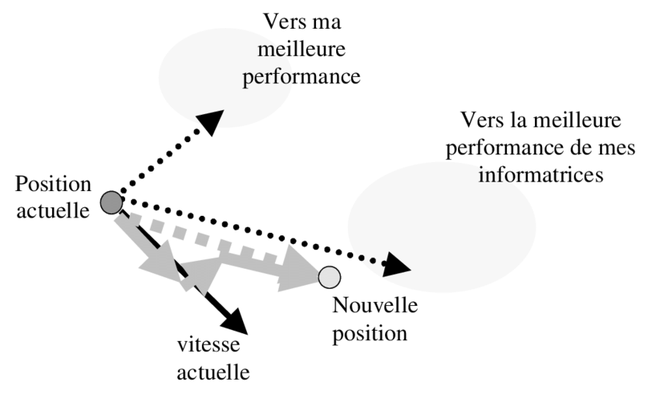
\includegraphics[scale=0.3]{dimension1.png}
			\end{figure}
   		 \column{5cm}
			\begin{figure}
 			\centering 
			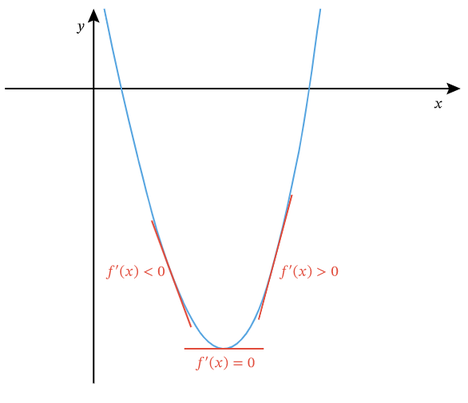
\includegraphics[scale=0.3]{dimension2.png}
      			\end{figure}
 	 	\end{columns}
	\end{frame}

	\begin{frame}[fragile]
	\frametitle{Study of the impact of the parameters on the convergence}
	\framesubtitle{Optimisation in higher dimensions (above five)}
		\begin{center}
		\begin{columns}
    		\column{4cm}
    			\begin{figure}
      				\centering
       				
\includegraphics[scale=0.3]{dimension3.jpg}
			\end{figure}
		\column{5cm}
			\begin{verbatim}
			20% of total iterations
			85% of total iterations
			\end{verbatim}
		\end{columns}
		\end{center}
	\end{frame}
	\begin{frame}
	\frametitle{\color{velvet} Study of the impact of the parameters on the convergence}
	\framesubtitle{Evolution of ERJ in regard of the value of K | Rastrigin}
	ERJ in regard of K for the Rastrigin function
	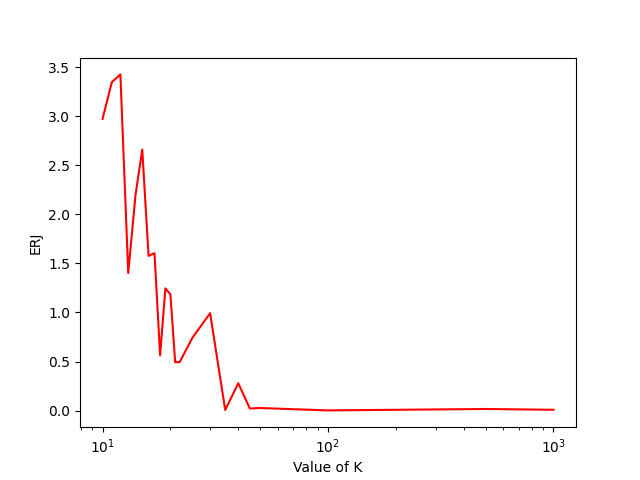
\includegraphics[scale=0.5]{Graphs/7.png}
	\end{frame}
	\begin{frame}
	\frametitle{\color{velvet} Study of the impact of the parameters on the convergence}
	\framesubtitle{Evolution of ERJ in regard of the value of K | Booth}
	ERJ in regard of K for the Booth function
	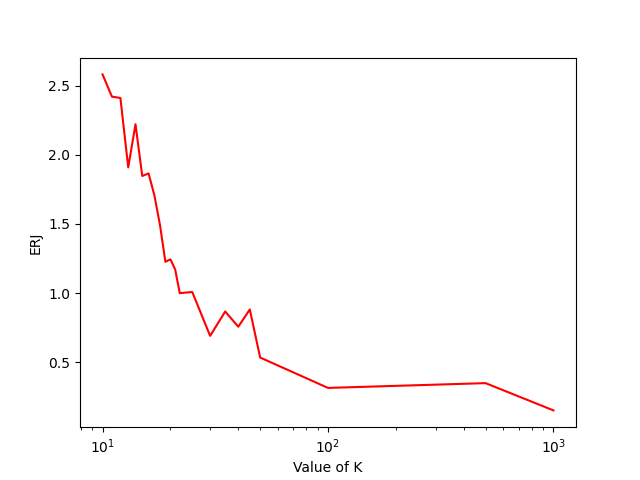
\includegraphics[scale=0.5]{Graphs/8.png}
	\end{frame}
	\begin{frame}
	\frametitle{\color{velvet} Study of the impact of the parameters on the convergence}
	\framesubtitle{Evolution of the average k in regard of the value of P | Rastrigin}
	Average k in regard of P for the Rastrigin function
	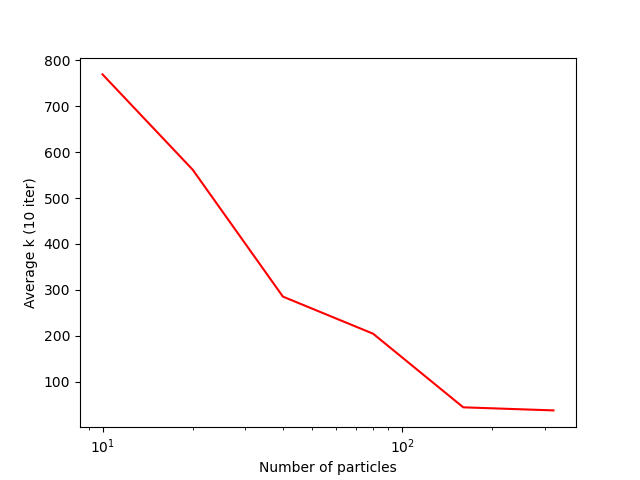
\includegraphics[scale=0.5]{Graphs/9.png}
	\end{frame}
	\begin{frame}
	\frametitle{\color{velvet} Study of the impact of the parameters on the convergence}
	\framesubtitle{Evolution of the average k in regard of the value of P | Booth}
	Average k in regard of P for the Booth function
	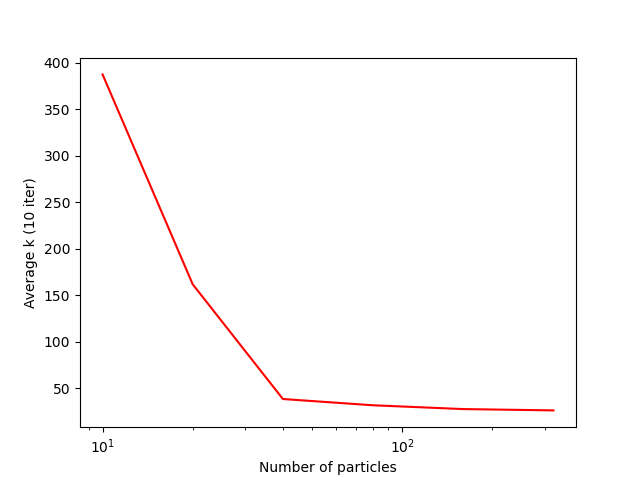
\includegraphics[scale=0.5]{Graphs/10.png}
	\end{frame}

	\begin{frame}
		\frametitle{\color{velvet} Annexes}

		\href{https://colab.research.google.com/drive/1-OzHX9b747wIw_0KCM51-NRGmR76BHQu?usp=sharing}{\color{velvet} Open the annex notebook in Colab} \\
		\href{https://github.com/Antix5/PSOchaos}{\color{velvet} Open the github repository with all the other documents}


	\end{frame}


	
	

\end{document}


